\graphicspath{{chapters/images/03/}}

\chapter{Next generation sequencing}

\section{Introduction}
Next generation sequencing is the gold standard for sequencing nowadays.
A series of discoveries allowed for the development of this technology:

\begin{multicols}{2}
    \begin{itemize}
        \item $1959$: first homogeneous DNA purified.
        \item $1970$: first discovery of type $II$ restriction enzymes.
        \item $1972$: first RNA gene sequence published.
        \item $1975$: Sanger publishes his plus-minus method of sequencing, unable to distinguish homopolymers.
        \item $1977$: Maxam and Gilbert publish their method that could distinguish homopolymers.
        \item $1977$: Sanger publishes the dideoxy-sequencing method.
    \end{itemize}
\end{multicols}

    \subsection{Progresses of sequencing}
    As can be seen in the graph \ref{moore} the cost of DNA sequencing is decreasing by a greater rate than the one predicted by Moore's law.
    This allows for greater number of samples and the sequencing of a different number of genomes.

    \begin{figure}[h]
        \centering
        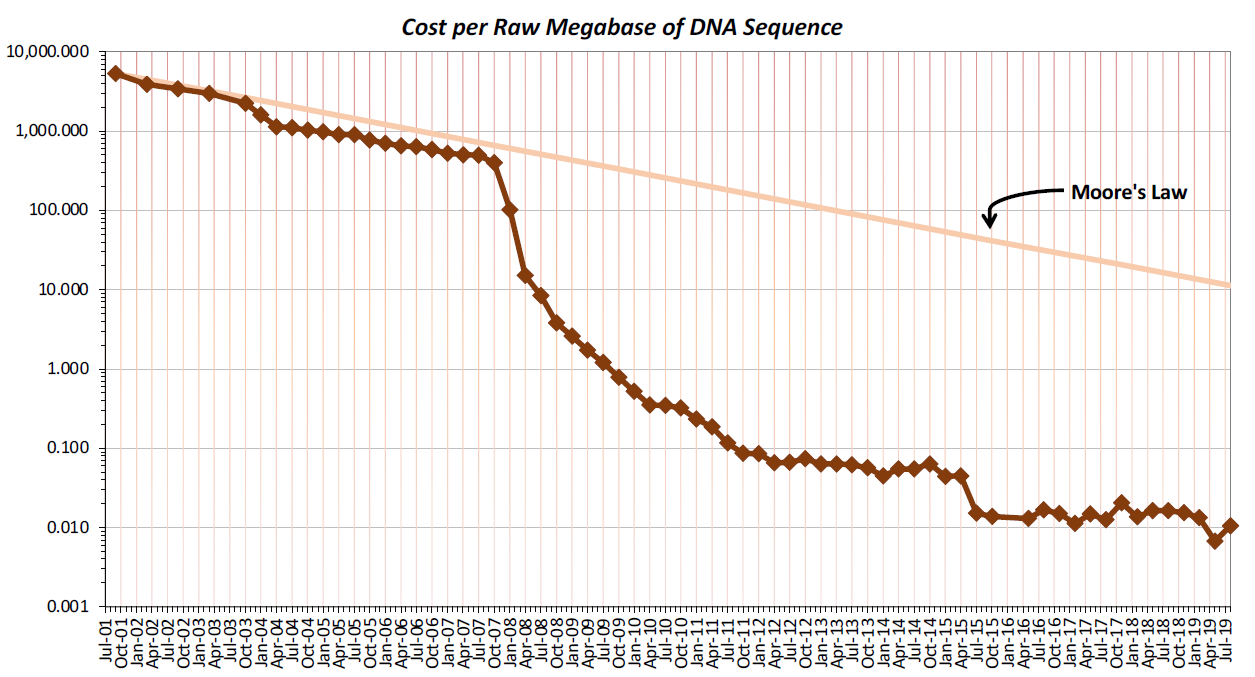
\includegraphics[width=0.6\textwidth]{sequencingCost}
        \caption{}
        \label{moore}
    \end{figure}

    \subsection{Methods of sequencing}
    The methods of sequencing can be grouped in three groups:

    \begin{multicols}{2}
        \begin{itemize}
          \item Chemical degradation of DNA: like the method of Maxam-Gilbert.
          \item Sequencing by synthesis (“SBS”): the most common approach and the first to be developed.
              It uses DNA polymerases in primer extension reactions.
              This technology is used by Illumina, Pacific Bioscences, Ion Torren and 454.
          \item Ligation-based: sequencing using short probes that hybridize to the template.
              This technology is used by SOLiD and Complete Genomics.
          \item Others like nanopores.
        \end{itemize}
    \end{multicols}

    \subsection{The Chain Terminators}

    \begin{figure}[H]
        \centering
        \begin{subfigure}[b]{0.49\textwidth}
            \centering
            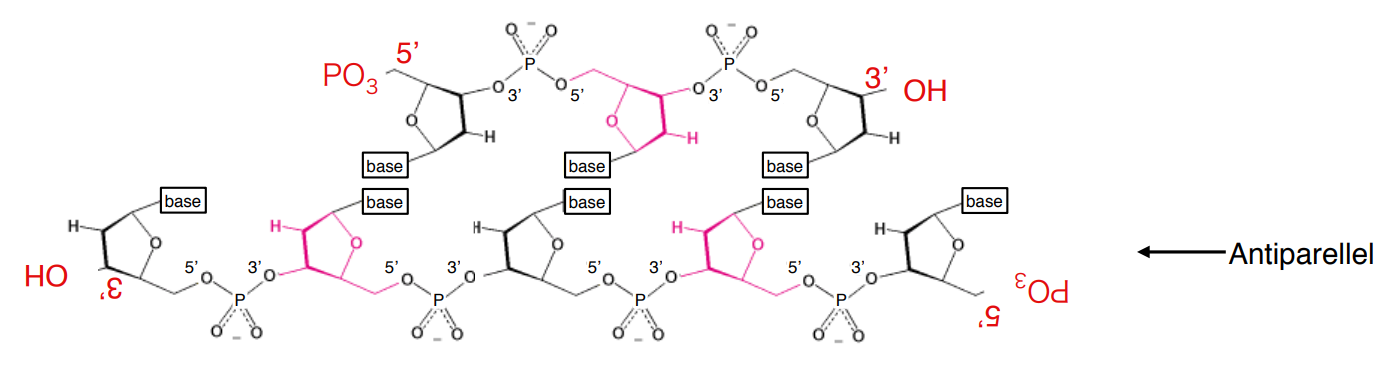
\includegraphics[width=\textwidth]{DNA-molecule}
            \caption{Normal DNA molecule, with oxydrilic group ligated to $3'$-ends}
            \label{normalDNAaddition}
        \end{subfigure}
        \hfill
        \begin{subfigure}[b]{0.49\textwidth}
            \centering
            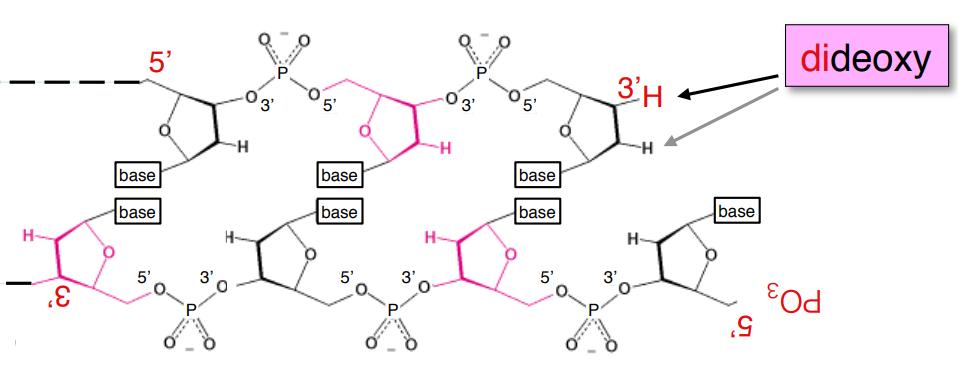
\includegraphics[width=\textwidth]{chain-term}
            \caption{Figure representing the difference between a normal DNA chain and one with chain terminators}
            \label{ChainTerm}
        \end{subfigure}
        \caption{Normal DNA synthesys \textit{vs} Chain terminators}
    \end{figure}

    Normally, the addition of new nucleotides to a generated molecule of DNA happens with the $3'$-end of the nucleotide chain \ref{normalDNAaddition}.
    Chain terminators are dideoxy nucleotides, ddNTPs, that cannot be further extended.
    These nucleotides don't have the oxydrilic group at their $3'$-end, so the DNA polymerase cannot further add other nucleotides to the chain \ref{ChainTerm}.

\section{Sanger method}

\begin{figure}[h]
    \centering
    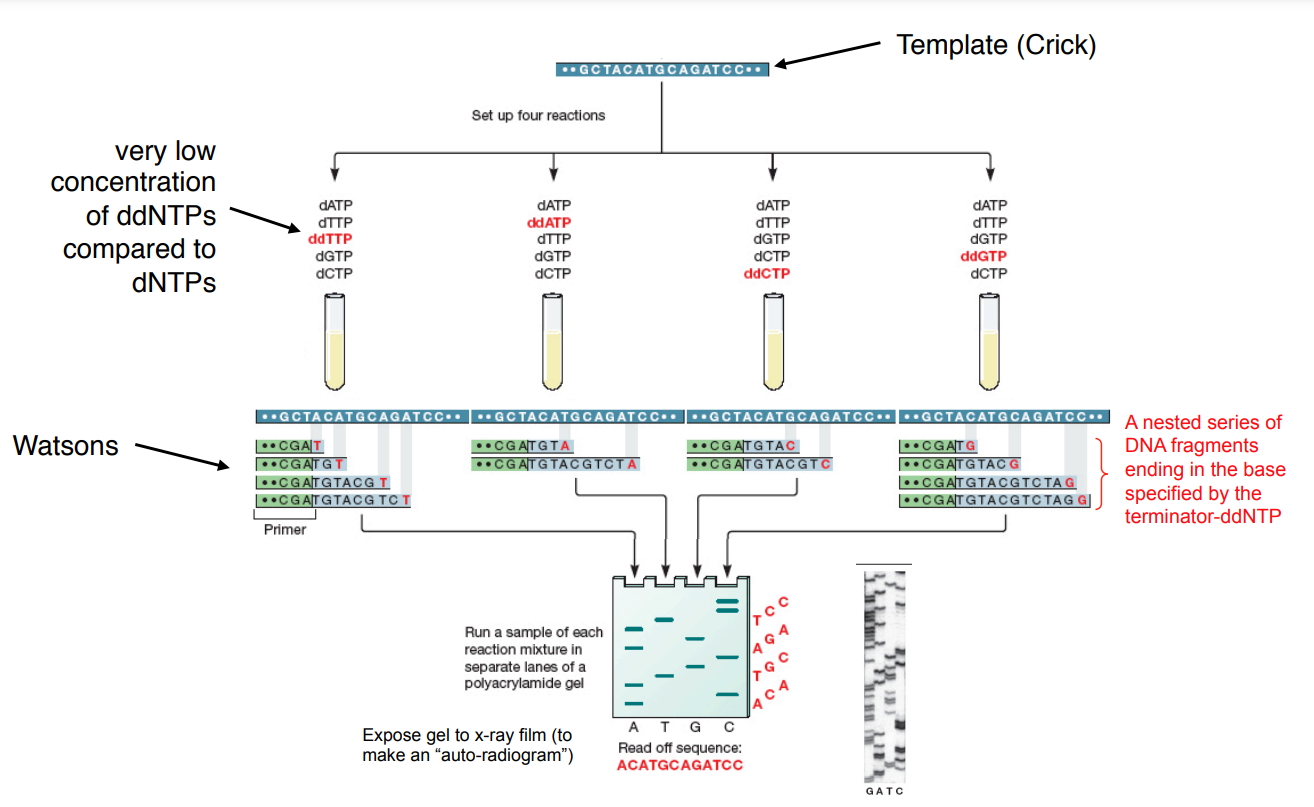
\includegraphics[width=\textwidth]{Sanger}
    \caption{Sanger's method process}
    \label{Sanger}
\end{figure}

The first method ever used to sequence DNA was designed by Frederick Sanger.
The Sanger manual sequencing system consists in an \textit{in vitro} process described in figure \ref{Sanger}.
It is also named a primer extension method.
It is performed over a single-filament DNA sample, and it uses chain terminators nucleotides, one for each type of nucleobase: ddATP, ddGTP, ddTTP, ddCTP.
The reaction is done inside four different reactions tubes, each containing:

\begin{multicols}{2}
    \begin{itemize}
        \item The sample DNA to be reproduced.
        \item A DNA polymerase.
        \item The normal nucleotides.
        \item One of the four possible chain terminator marked with sulfur-35.
            In each tube, the corresponding dideoxy-nucleotide was used with a concentration 10 times lower than the other normal nucleotides.
    \end{itemize}
\end{multicols}
The polymerization reactions produces several molecules of DNA with different length: each replicative cycle is terminated after the addition of a chain terminator nucleotide.
The initial DNA sequence is reconstructed using a long PAGE gel with high concentration of urea ($6 - 7 M$) to avoid the coiling of the DNA single-filaments.
High voltages are required to achieve a highly risolutive run.
This high resolution was needed as DNA's fragments are different only for a nucleotide.
After having run it the bands were visualized through auto-radiography in order to evidentiate the phosphorescent signals.

The sequence is read starting from the shortest fragments at the end of the gel and going up along it, looking for the first presence of a band in one of the four runs.

    \subsection{Automatic sequencing}
    To automatize the Sanger methods fluorescent proteins substituted the radioactive signal.
    Several versions were developed:

    \begin{multicols}{2}
        \begin{enumerate}
          \item Fluorescent primers marked with a single fluorochrome.
          \item Four aliquotes of the same primer were used marked with four different fluorochromes, able to emit different fluorescences.
          \item Four different fluorochromes were used to mark the single ddNTPs
        \end{enumerate}
    \end{multicols}

    Thanks to the use of 4 different fluorochromes, it was possible to use a single electrophoretic lane to carry the sequencing reaction.
    Also a cyclic replicative reaction was performed with this procedure using a thermal cycler:

    \begin{multicols}{2}
        \begin{enumerate}
          \item Denaturation at $95$°C of the DNA to be sequences
          \item Annealing at $50-70$°C of the primer specific to one of the two filaments
          \item Extension at $72$°C by using a \textit{Taq}-polymerase to avoid the formation of coiled structures in the DNA molecule to be sequenced.
        \end{enumerate}
    \end{multicols}

    The resulting molecules are run through a long PAGE gel and fluorescence is triggered irradiating the DNA molecules.

    \begin{figure}[h]
        \caption{}
        \centering
        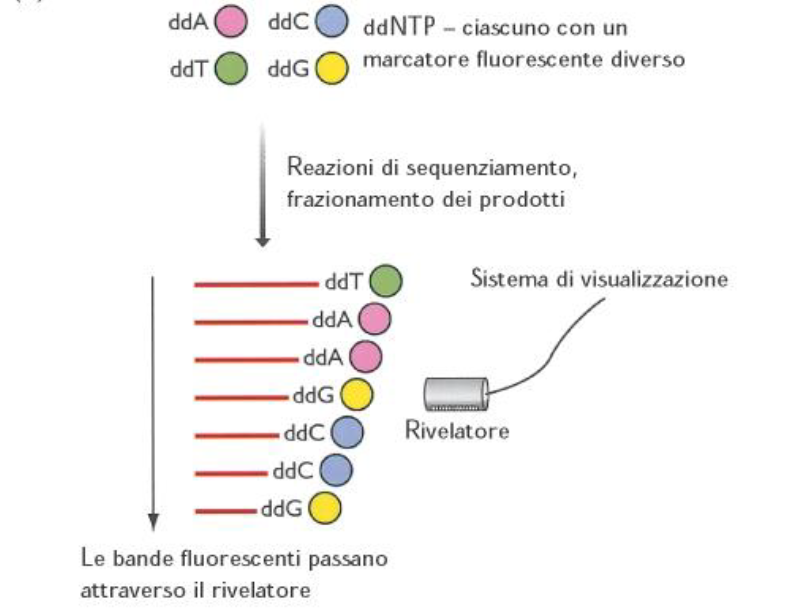
\includegraphics[width=0.8\textwidth]{automaticSang}
        \label{}
    \end{figure}

    More usefully, this sequencing method is performed by using a capillar filled with a synthetic polymer with the same function of polyacrillamide.
    The analysis produces an electropherogram, with a color depicting the probability of each base being in each position.
    The electropherogram is refined through algorithms that can boost the signal to noise ration, correct the dye effect and reduce all systematic errors.

        \begin{figure}[h]
        \caption{}
        \centering
        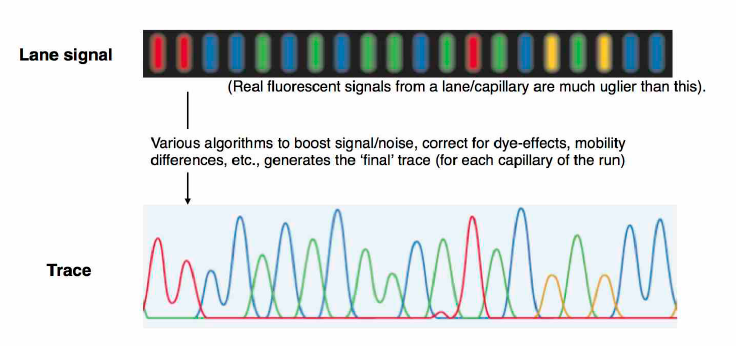
\includegraphics[width=0.8\textwidth]{elettroferogramma}
        \label{}
    \end{figure}

    \begin{figure}[h]
        \centering
        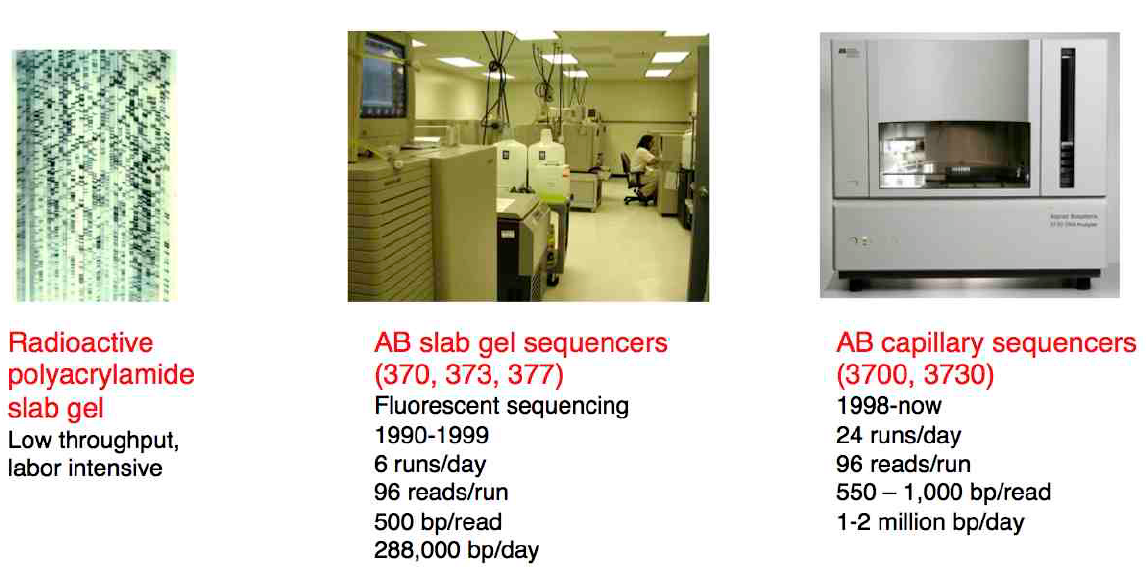
\includegraphics[width=0.8\textwidth]{progressSangerMachines}
        \caption{The implementation of capillary sequencing machines gave the possibility to make more runs than with the others.
                    $\sim 1000$ fold productivity increase was allowed
                }
        \label{}
    \end{figure}

    The Sanger automatic sequencing method was used extensively for the majority of the human project.

\section{Development of Sequencing Machines}
The method used for sequencing has to be chosen based on the wanted output, like the quality required and the type of input.
Different technologies have different strengths and weaknesses:

\begin{multicols}{2}
    \begin{itemize}
        \item SOLID sequences reads long only $35$-$75$ bases and it is not used anymore.
        \item Sanger sequencing, or the capillary, can read up to $1000$ bases, but has a low throughput.
        \item MINION allowed to sequence an entire genome of \textit{E. coli}.
    \end{itemize}
\end{multicols}

A plethora of sequencing machines are available today.
None of them is able to sequence DNA directly from a sample, requiring different preparation step.
Today machines producing high-throughput output of short reads are preferred.

\begin{figure}[H]
\centering
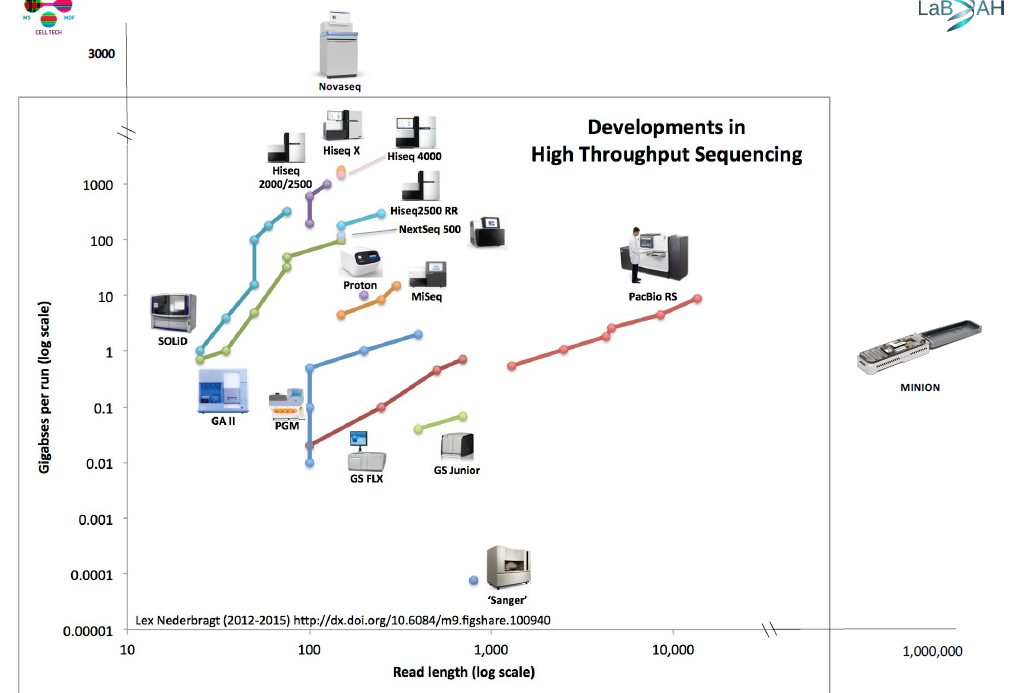
\includegraphics[width=1\textwidth]{sequencingMachines}
\caption{It can be noticed how recent developments had the scope of increasing the output data}
\label{}
\end{figure}

The most wide-spread machines are from ILLUMINA like NovaSeq.
They use sequencing by synthesis and they amplify the signal through the use of clusters.

\begin{figure}[H]
\centering
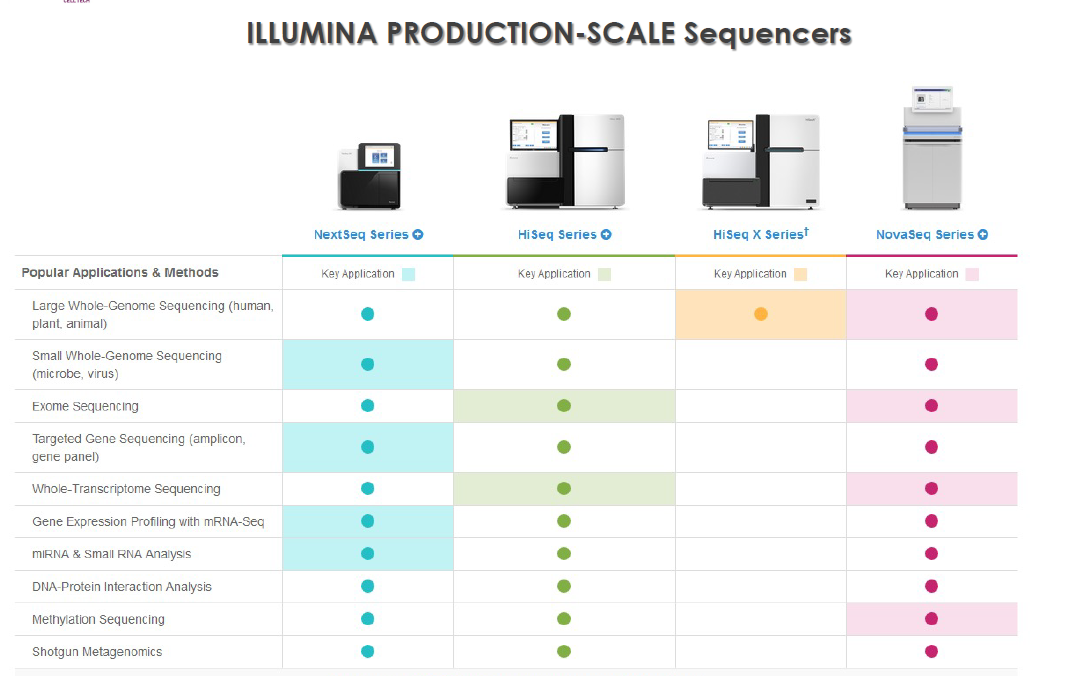
\includegraphics[width=0.8\textwidth]{sequencingMachinesIllumina}
\caption{}
\label{}
\end{figure}

\section{Next Generation Sequencing}
The NGS protocol requires $3$ steps:

\begin{multicols}{2}
    \begin{enumerate}
          \item Sample preparation: series of fragments added.
          \item Clonal amplification: needed to replicate fragments attached to the solid surfaces, since machines are not sensible to single molecules.
          \item Sequencing: ILLUMINA sequencing is one of the techniques used to obtain sequence data nowadays.
    \end{enumerate}
\end{multicols}

$3^{rd}$ generation allow to read a molecule without replicating it.

    \subsection{ILLUMINA sequencing}

        \subsubsection{Fragments and Library preparation}
        During fragmentation the DNA or RNA polymers that need to be sequenced are fragmented in short read sequences.
        This is because the machines are able to sequence only read with a length of a few hundred nucleotides.
        These fragments need to be tagmented: in this process one or two indexes, or barcodes are added to the fragment so that it has two sequencing primer binding sites and regions complementary to the oligonucleotides in the chamber.
        Indexes allow to distinguish between sample and, in the case of pair end sequencing, allow to distinguish between the forward and reverse read.

        \begin{figure}[h]
            \centering
            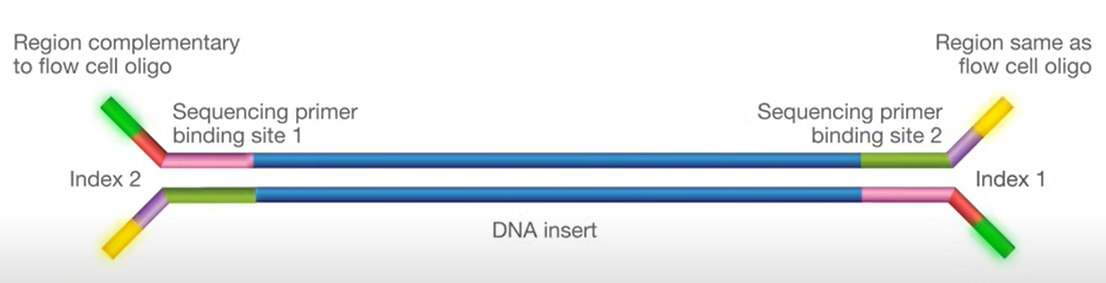
\includegraphics[width=0.8\textwidth]{tagmentedFragments}
            \caption{Figure representing the a good prepeared fragment, it has two indexes, two sequencing primer binding sites and regions complementary to the oligonucleotides present in the chamber}
            \label{}
        \end{figure}

        \subsubsection{Clonal amplification and ILLUMINA sequencing procedure}

        \begin{figure}[h]
            \centering
            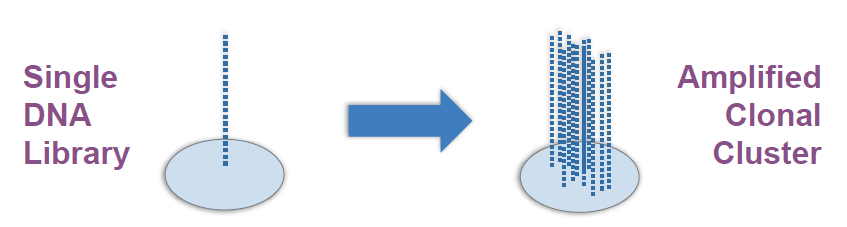
\includegraphics[width=0.6\textwidth]{clusterAmplification}
            \caption{}
            \label{clusters}
        \end{figure}

        Clonal amplification is necessary to amplify the signal from each fragment.
        ILLUMINA machines make use of clusters to sequence DNA: group of DNA strand positioned near each other that generate from a single fragment.
        Each cluter represents thousands of copies of the same DNA strand in a $1$-$2\mu m$ spot \ref{clusters}.

        \begin{figure}[h]
            \centering
            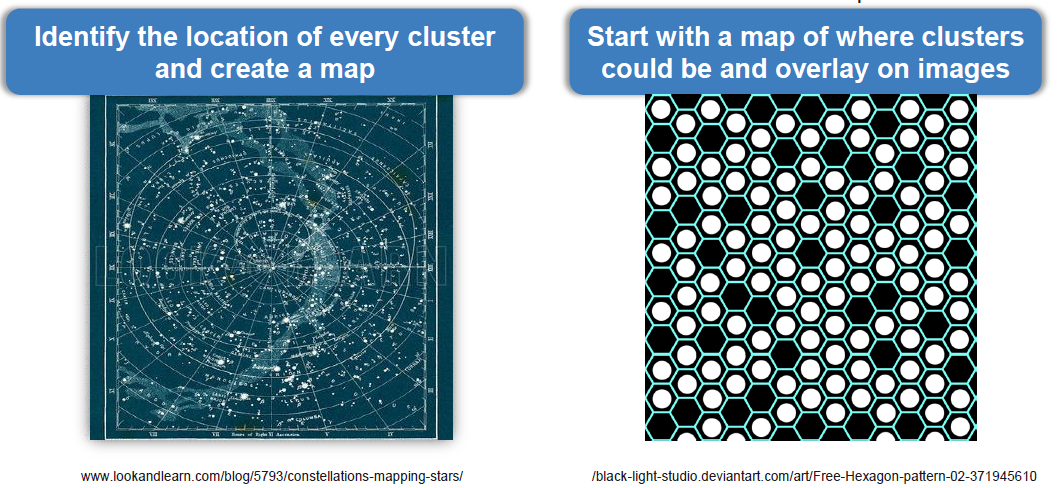
\includegraphics[width=0.8\textwidth]{rigidGeneration}
            \caption{}
            \label{rigid}
        \end{figure}

        The clonal amplification process happens in flow cells, slides of glass in which fragments flow over channels.
        Changes in temperature allow for ligations and separations.
        The surface of the cells is functionalized with a series of oligos complementary to library adapters.
        These flow cell can be patterned (cluster in specific positions) or random (cluster randomly positioned).
        In the former the location of the cluster can be known (rigid registration \ref{rigid}) or unknown.

        \begin{figure}[h]
            \centering
            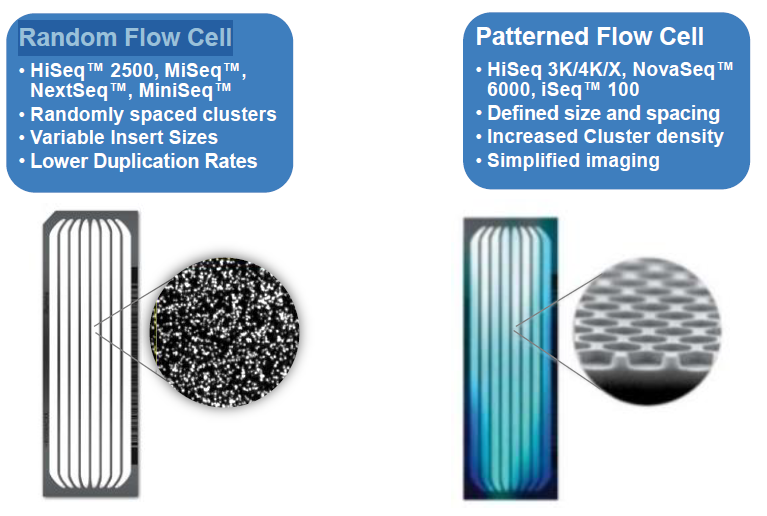
\includegraphics[width=0.6\textwidth]{randomPatternCells}
            \caption{}
            \label{}
        \end{figure}

        \subsubsection{Fragment attachment to the clusters}
        Once the fragments start flowing over the chambers, they can bind only to one of the two oligos functionalizing the plate.
        Once they are attached to the surface the sequencing process is controlled through solvents and temperature.
        As shown in \ref{singDoubInd} the sequencing process differs between single end and paired end sequencing.

        \begin{figure}[H]
            \centering
            \begin{subfigure}[b]{0.39\textwidth}
                \centering
                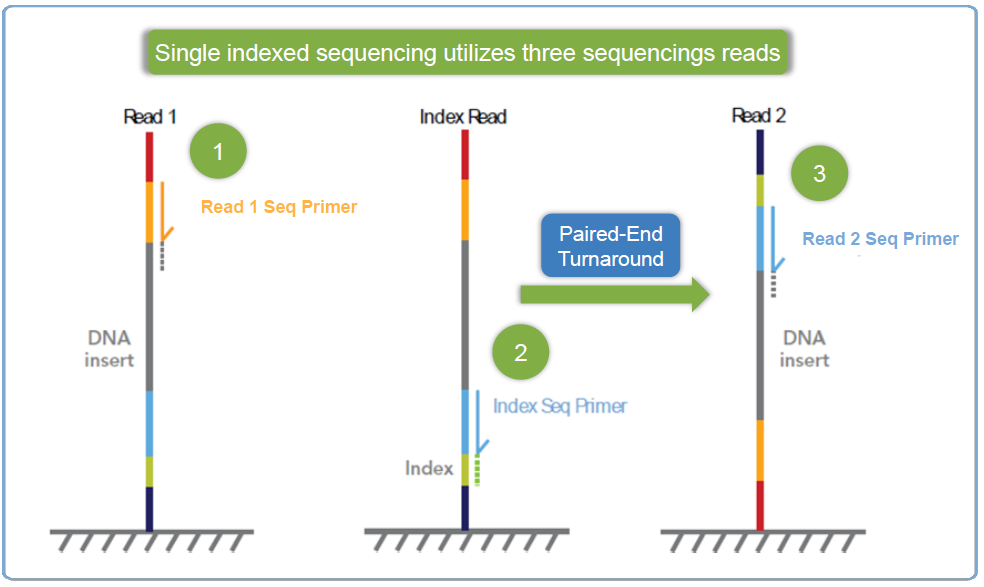
\includegraphics[width=\textwidth]{singleIndex}
                \caption{single index}
            \end{subfigure}
            \hfill
            \begin{subfigure}[b]{0.60\textwidth}
                \centering
                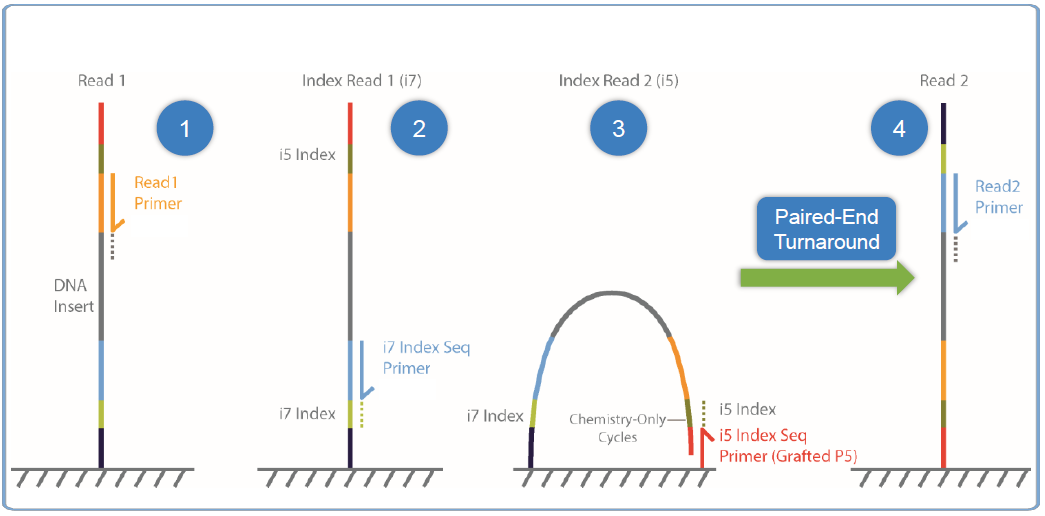
\includegraphics[width=\textwidth]{doubleIndex}
                \caption{double index}
            \end{subfigure}
            \caption{Single/double index for ILLUMINA sequencing}
            \label{singDoubInd}
        \end{figure}

        \subsubsection{Sequencing}

        \begin{figure}[H]
            \caption{}
            \centering
            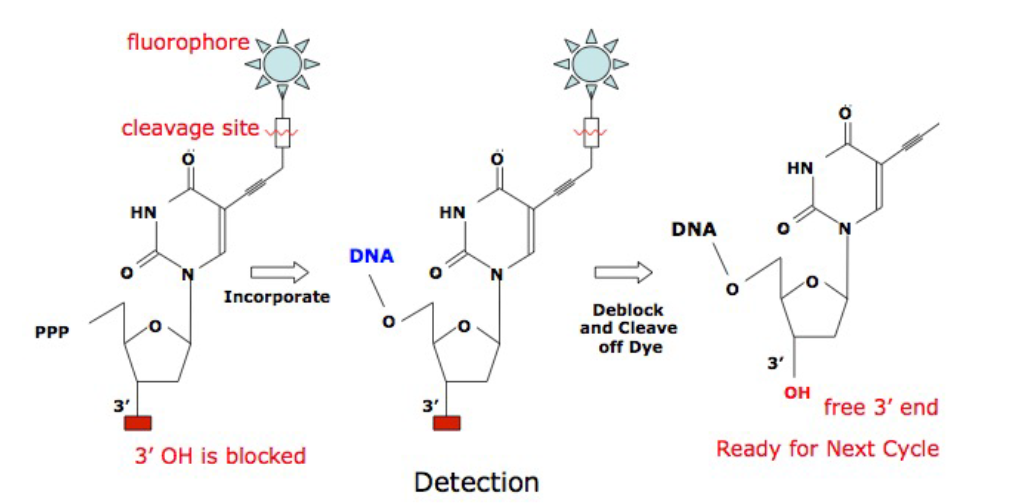
\includegraphics[width=0.7\textwidth]{ILLUMINArev}
            \label{ILLUMINArev}
        \end{figure}

        Reversible terminators \ref{ILLUMINArev} allow a real time analysis of the sequencing through the syntheses reaction.
        The fluorophore part of the terminator can be cleaved to eliminate the signal.

        \begin{figure}[h]
        \caption{}
        \centering
        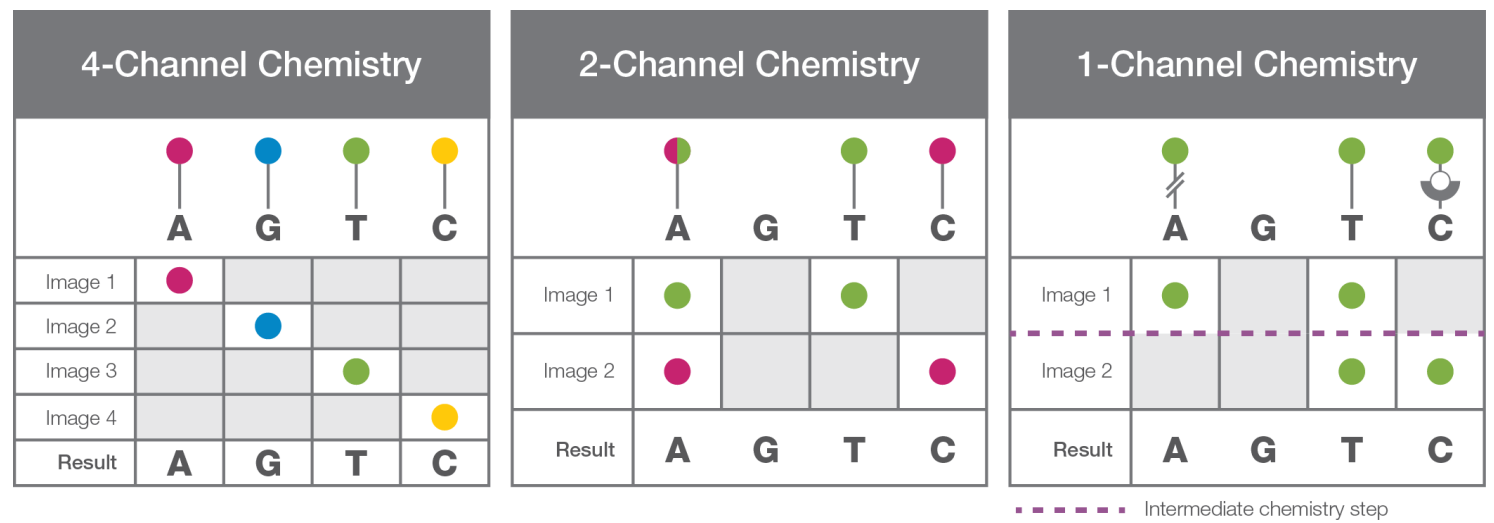
\includegraphics[width=0.8\textwidth]{ChannelILLUMINA}
        \label{ChannelILLUMINA}
        \end{figure}

        Depending on the number of fluorescent molecules used ILLUMINA sequencers are distinguished in the $4$-channel, $2$-channel or $1$-channel type.
        In the case of the $4$-channel $4$ images are taken in each cycle and each cluster apperas in only one of the four images \ref{ChannelILLUMINA}.
        The highest intensity base in a cluster is the called base for that cluster.
        In case no base is clearly related to a position the base calling returns $N$.
        This reading process can be done through single end reads on a single extreme of the fragment or through paired-ends reading, where each fragment is read in a forward and reverse way.
        This latter method gives structural information.

    \subsection{Pacific Bioscience}
    In the Pacific Bioscience PacBio sequencer the long DNA filament to be sequenced is attached to a polymerase, over the surface of a SMRT (Single Molecule Real Time) cell.
    This cell is really small, and at each nucleation process a light signal is emitted.
    The produced light is not able to get out of the walls, and its duration is extremely restricted.
    The registration of the light signal correspond to a base calling.
    Its main advantage over ILLUMINA is the possibility of sequencing really long DNA molecules.

    \begin{figure}[H]
    \centering
    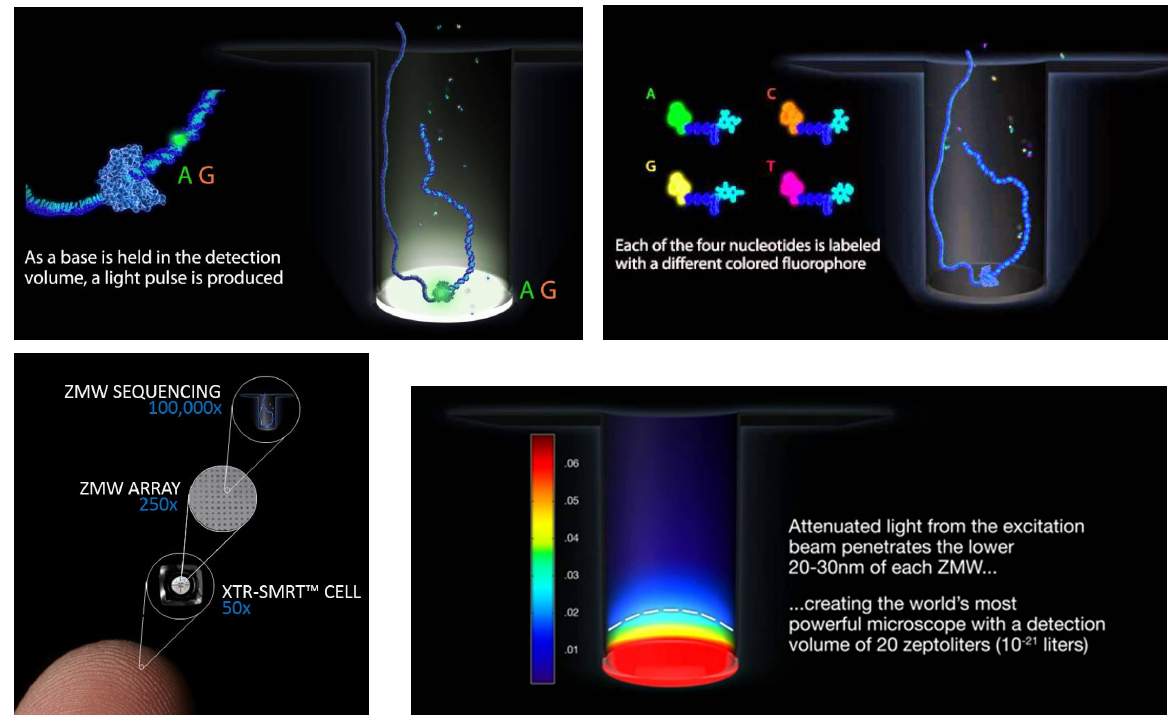
\includegraphics[width=1\textwidth]{PacBIO}
    \caption{}
    \label{}
    \end{figure}


\subsection{Nanopore sequencing}
In nanopore sequencing the sequence is detected through the passage of DNA molecule into intramembrane protein.
This produces a voltage changes that corresponds to a base calling.
This technology is in constant development and is not widely used because of the, although improving, high error rate.
